% Generated by plsimcount.pffigure -- do not edit; regenerate instead.
% figure: A-tte-by-order -- Suzuki formulas of each order, r from: Commutator bound (2021)
% source: results/np-main/seed1/results.json
% metric=cnot gatebase=cz merged
% seed=1 t=n template=simcount synth=pygridsynth
% git_commit=01d3c275ceae2840002bd1aaea68f59b987c4975 git_dirty=False
% source_sha256=0dd1c9775f148df550d3d3f68cfeee1d2d060b7913324535bbf1533b52b4d2c2
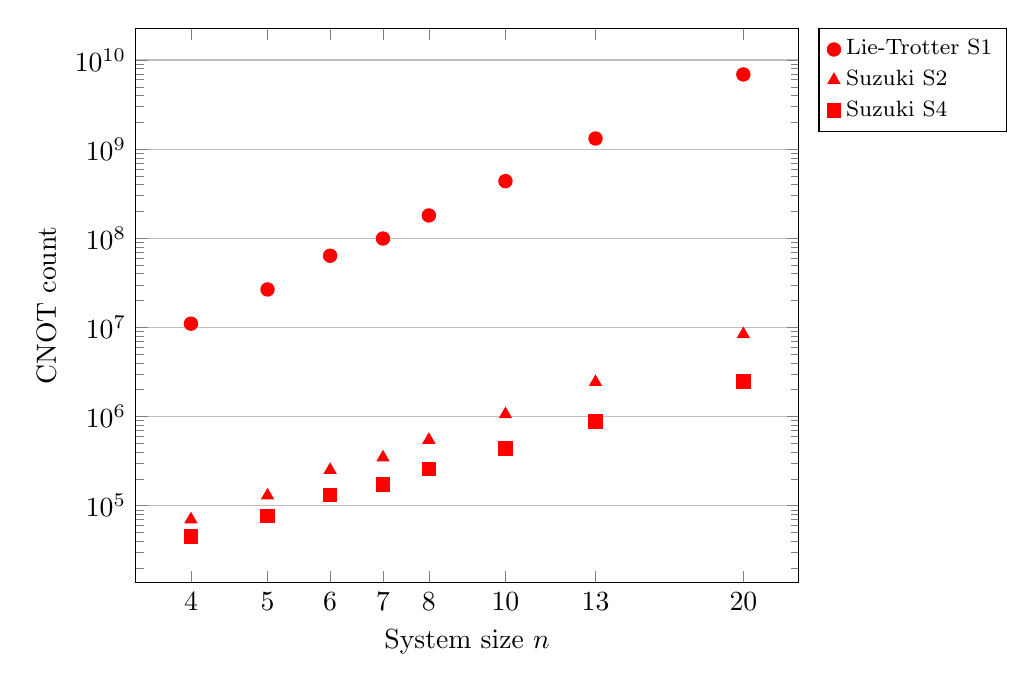
\begin{tikzpicture}
  \begin{loglogaxis}[
    width=10cm,
    xlabel={System size $n$},
    ylabel={CNOT count},
    xtick={4,5,6,7,8,10,13,20},
    xticklabels={4,5,6,7,8,10,13,20},
    ymajorgrids=true,
    legend pos=outer north east,
    legend cell align=left,
    legend style={font=\footnotesize},
  ]
    \addplot[only marks, red, mark=*, mark size=2.4pt, mark options={solid, fill=red}] coordinates {
      (4,11020296)
      (5,26672070)
      (6,63716940)
      (7,99335082)
      (8,180316560)
      (10,437836740)
      (13,1315943928)
      (20,6887318520)
    };
    \addlegendentry{Lie-Trotter S1}
    \addplot[only marks, red, mark=triangle*, mark size=2.4pt, mark options={solid, fill=red}] coordinates {
      (4,70120)
      (5,130200)
      (6,251520)
      (7,347830)
      (8,546880)
      (10,1061300)
      (13,2436330)
      (20,8383600)
    };
    \addlegendentry{Suzuki S2}
    \addplot[only marks, red, mark=square*, mark size=2.4pt, mark options={solid, fill=red}] coordinates {
      (4,45024)
      (5,76230)
      (6,131040)
      (7,173754)
      (8,257040)
      (10,437220)
      (13,884520)
      (20,2469600)
    };
    \addlegendentry{Suzuki S4}
  \end{loglogaxis}
\end{tikzpicture}
